\documentclass{beamer}
\synctex=1

% Die folgende Anweisung kompiliert nur bestimmte frames,
% wodurch das Kompilieren u.U. deutlich schneller wird.
% Das kann bei langen Präsentationen wärend des Erstellens einige Zeit sparen.

% \includeonlyframes{ctl}

\usepackage[utf8]{inputenc}
\usepackage[ngerman]{babel}
\usepackage[T1]{fontenc}
\usepackage{graphicx}
\usepackage{verbatim}
\usepackage{csquotes}
\usepackage{eurosym}
\usepackage{wasysym}
\MakeAutoQuote{„}{”}
\usepackage[absolute,overlay]{textpos} % für \textblock

\usepackage{fancyvrb}
\usepackage{newverbs}
\usepackage{xcolor}

% Serifen-Freie Schrift für den Normalen Text ist gut,
% aber für Formeln wollen wir schöne Serifen (sieht besser aus)
\usefonttheme[onlymath]{serif}

\definecolor{myblue}{rgb}{0.3,0.5,0.8}

% Die Standard-Einstellungen des hyperref-paketes haben bewirken
% sehr grelle Fraben. -> Anpassung
\hypersetup{
  colorlinks=true,
  linkcolor=, %
  urlcolor=[rgb]{.2, .2, .5} %
  % allcolors=[rgb]{0, 0, 0} % schwarz
}



\usetheme{Dresden}
\setbeamertemplate{navigation symbols}{}
\setbeamertemplate{footline}[frame number]

% In jedem Frame soll das FSFW-Logo angezeigt werden:
\addtobeamertemplate{frametitle}{}{%
  \begin{textblock*}{130mm}(.963\textwidth,8.4mm)
    \includegraphics[width=2.25cm]{img-src/fsfw-logo.pdf}
  \end{textblock*}
}


\title{Eine Präsentation mit der \LaTeX-beamer-Klasse}
\subtitle{(Eine Alternative zu Powerpoint etc.)}

%##############################################################################
%##############################################################################

\begin{document}

\begin{frame} % Das ist die Titelfolie
  \begin{center}%
    \includegraphics[width=3cm]{img-src/fsfw-logo-with-text.pdf}\\

    \vspace*{-0.5\baselineskip}

    \parbox{.95\columnwidth}{\centering\Large\inserttitle}

    \vspace*{\baselineskip}

    \structure{\large \insertsubtitle}
  \end{center}
\end{frame}



%%%%%%%%%%%%%%%%%%%%%%%%%%%%%%%%%%%%%%%%%%%%%%%%%%%%%%%%%%%%%%%%%%%%%%%%%%%%%%%%


\begin{frame}[label=beamer]
  \frametitle{Übersicht}

Was kann das Beamer-Paket?
  \begin{itemize}
  \item Bildschirm-Präsentationen (PDF) mit \LaTeX{}-Code erzeugen
  \pause
  \item Alle Vorteile von \LaTeX
  \begin{itemize}
   \item Sehr guter Formelsatz, z.B. $\int_0^1\left(\sum_{i=1}^n \omega_i(t \mathbf x) x_i\right)dt$
   \item Quelldaten: reiner Text $\rightarrow$ gut für Zusammenarbeit
  \end{itemize}
 \end{itemize}

  \bigskip
  
  \pause
Effekte?
\begin{columns}
% leere Spalte, um die anderen beiden nach rechts zu schieben
\column[t]{0.1\textwidth}
~

\column[t]{0.5\textwidth}
  \begin{itemize}
    \item Möglichkeiten überschaubar\\
    (keine fliegenden Folien)
    
    \pause
    
    \item aber einiges \visible<5->{geht} immerhin
    \pause
    \pause
    \item {\color<7>{myblue}außerdem sollten Effekte sparsam eingesetz werden}
    \end{itemize}
%

\column[t]{0.05\textwidth}
% leere Spalte als Abstandshalter
~

\column[t]{0.55\textwidth}

\pause
\pause

Zum Erklären von "`komplizierten"' Sachen reicht es:\\[2em]


$\Gamma =\lambda
	\Big(
           \only<8>{\sin(x)^2 + \cos(x)^2}
           \only<9->{\underbrace{\sin(x)^2 + \cos(x)^2}_{= 1}}
	\Big)
	\only<10->{=\lambda}
       $
%  
\end{columns}
\end{frame}

%%%%%%%%%%%%%%%%%%%%%%%%%%%%%%%%%%%%%%%%%%%%%%%%%%%%%%%%%%%%%%%%%%%%%%%%%%%%%%%%

\begin{frame}[label=wb]
\begin{center}
 \vspace{10mm}
\structure{\Huge  Praxisbeispiel einer Folie}\\
{\tiny(Aus anderem Vortrag kopiert)}
\end{center}

\end{frame}


%%%%%%%%%%%%%%%%%%%%%%%%%%%%%%%%%%%%%%%%%%%%%%%%%%%%%%%%%%%%%%%%%%%%%%%%%%%%%%%%

\begin{frame}{FSFW – Freie Software und Freies Wissen}

% Hier werden zwei Spalten angelegt, als (schneller, aber fragwürdiger) Trick
% um horizontal mehr Platz zu erreichen.
% 
\begin{columns}

\column[t]{1\textwidth}
\vspace{-5mm}
  \begin{itemize}
  \item Hochschulgruppe seit 2014, ca. 10 Leute (TU, HTW, …)
  \item Warum machen wir das? Aus Überzeugung!

  \begin{itemize}
  \item \emph{Überzeugung 1}: freie und quelloffene Software ist (oft) besser\\
    (technische + nicht technische Argumente)\\
    \bigskip
    \pause
  \item \emph{Überzeugung 2}: öffentlich finanzierte wissenschaftliche Inhalte
    (AutorInnen, GutachterInnen) sollten nicht von öffentlich finanzierten
    Bibliotheken für horrende Summen von Zeitschriften-Verlagen gekauft werden
    müssen
  \end{itemize}

    \pause
  \item Bisherige Projekte
    \begin{itemize}
    \item Linux-Install-Party, Linux-Presentation-Day
    \item Monatliche \href{https://fsfw-dresden.de/sprechstunde}{Sprechstunde} zu \LaTeX{} u.a.
    \item Programmpapier, \href{https://fsfw-dresden.de/git-ws}{git-Workshop}
    \item \textbf<4-5>{„Uni-Stick”:~80 $\times$ 8\,GB mit freier Software}
    \item Verschlüsselungsgewinnspiel
    \end{itemize}
    \pause
    \pause
    \pause
    \item Für (Mitmachen-)Interessierte: \url{https://fsfw-dresden.de}
  \end{itemize}

  
% Die zwei Bilder sollen auf dem Frame erst in Stufe 4 bzw. 5 angezeigt werden.

% Die textblock-Umgebung erlaubt absolute Positionierung
% (Nachteil: Wenn sich der Inhalt ändert, muss manuell nachgesteuert werden).
\begin{textblock*}{5cm}[0.,0.](90mm,63mm)
\only<4>{
  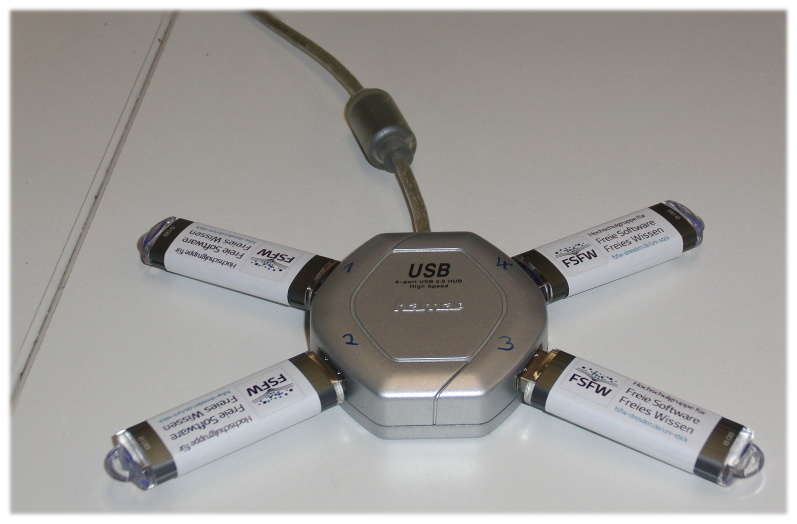
\includegraphics[width=35mm]{img-src/usb-hub}
}
\only<5->{
  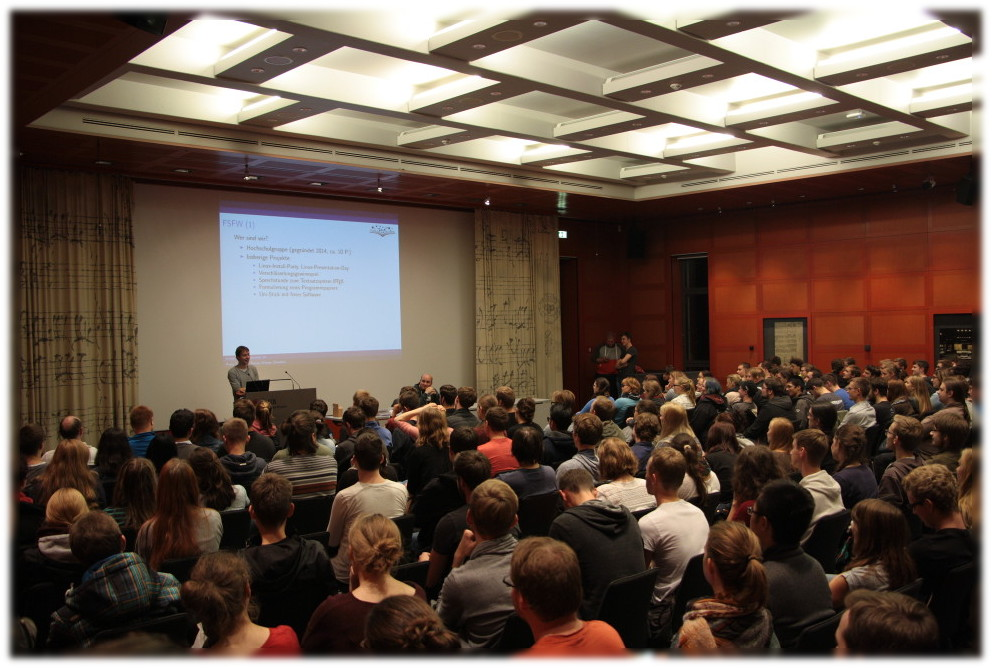
\includegraphics[width=35mm]{img-src/uni-stick-ausgabe-vortrag}
}
\end{textblock*}

% leere 2. Spalte mit 10% Seitenbreite -> bewirkt linksverschiebung der ersten Spalte
\column[t]{.1\textwidth}
~
\end{columns}
\end{frame}

%%%%%%%%%%%%%%%%%%%%%%%%%%%%%%%%%%%%%%%%%%%%%%%%%%%%%%%%%%%%%%%%%%%%%%%%%%%%%%%%

\begin{frame}[label=link10]{Quellen und Links (Auswahl)}
\tiny
\begin{itemize}
 \item \url{https://www.sharelatex.com/blog/2013/08/13/beamer-series-pt1.html}
 \item \url{http://www.mathematik.uni-leipzig.de/~hellmund/LaTeX/beamer2.pdf}
 \item \url{https://tex.stackexchange.com/questions/tagged/beamer}
% \url{https://learn.adafruit.com/an-introduction-to-collaborating-with-version-control/initializing-a-repository-and-making-commits}
\item ...
\end{itemize}
\end{frame}



\end{document}
